\chapter{Généralités sur les fonctions}

\section{Définition, vocabulaire et notations}

\begin{defin}[Fonction et ensemble de définition]
	Soit $\mathcal{D}$ un intervalle ou une réunion d'intervalles de $\R$.

	Une \textbf{fonction} $f$ définie sur $\mathcal{D}$ associe à tout nombre réel $x \in \mathcal{D}$ un \textbf{unique} nombre réel, noté $f(x)$.

	$\mathcal{D}$ est l'\textbf{ensemble de définition} de la fonction $f$, parfois noté $\mathcal{D}_f$.

	On note :
	\[
		f : \begin{array}[t]{rcc}
			\mathcal{D} & \longrightarrow & \R   \\
			x           & \longmapsto     & f(x)
		\end{array}
	\]

	On lit : \og{}$f$ est la fonction qui, à $x$, associe $f(x)$\fg{}.
	\begin{center}
		\begin{tikzpicture}[scale=0.75,>=Stealth,ensemble/.style={draw, thick, minimum width=3cm, minimum height=1.8cm, rounded corners=5pt, align=center}]
			\node[ensemble, black] (DF) at (0,0) {};
			\node[ensemble, blue!30!black] (R) at (9,0) {};
			\node[black, above=3pt, font=\large\bfseries] at (DF.north) {$\mathcal{D}_f$};
			\node[blue!30!black, above=3pt, font=\large\bfseries] at (R.north) {$\R$};
			\coordinate (X) at ($(DF.center) + (0.3, 0.6)$);
			\coordinate (FX) at ($(R.center) - (0.3, -0.6)$);
			\fill (X) circle (2.5pt) node[left=3pt, font=\large] {$x$};
			\fill (FX) circle (2.5pt) node[right=3pt, font=\large] {$f(x)$};
			\draw[->, ultra thick, black!70] ($(DF.east) + (0.2, 0.6)$) -- ($(R.west) - (0.2, -0.6)$) node[midway, above=4pt, black, font=\huge\bfseries] {$f$};
			\node[font=\small, black] at (4.5, -0.2) {associe un \textbf{unique} réel};
			\node[below, black] at (DF.south) {Ensemble de départ};
			\node[below, black] at (R.south) {Ensemble d'arrivée};
		\end{tikzpicture}
	\end{center}
\end{defin}

\begin{rem}
	$x$ représente la \textbf{variable}. $f$ est le nom de la fonction (la \og{}machine\fg{} mathématique) tandis que $f(x)$ est un nombre réel (le résultat de la transformation).
\end{rem}

\begin{methode}[Déterminer un ensemble de définition]
	Pour déterminer l'ensemble de définition d'une fonction donnée par une expression algébrique, on recherche les éventuelles \textbf{valeurs interdites} :
	\begin{itemize}
		\item Un dénominateur ne doit jamais être nul.
		\item Une expression sous une racine carrée doit toujours être positive ou nulle.
	\end{itemize}

	Déterminer l'ensemble de définition des fonctions suivantes :

	\begin{multicols}{3}
		\begin{enumerate}
			\item $f(x) = 2x^2 - 3x + 1$
			\item $g(x) = \dfrac{x+4}{2x-6}$
			\item $h(x) = \sqrt{3x + 12}$
		\end{enumerate}
	\end{multicols}

	\begin{correction}
		\nline
		\begin{enumerate}
			\item $f(x)$ est définie pour tout réel $x$. Il n'y a ni fraction ni racine carrée. Ainsi, $\mathcal{D}_f = \R$.
			\item $g(x)$ existe si et seulement si son dénominateur n'est pas nul :
			      \[
				      2x - 6 = 0 \iff 2x = 6 \iff x = 3
			      \]
			      La valeur $3$ est une valeur interdite. Ainsi, $\mathcal{D}_g = \R \setminus \{3\} = \intoo{-\infty}{3} \cup \intoo{3}{+\infty}$.
			\item $h(x)$ existe si et seulement si la quantité sous la racine est supérieure ou égale à zéro :
			      \[
				      3x + 12 \ge 0 \iff 3x \ge -12 \iff x \ge -4
			      \]
			      Ainsi, $\mathcal{D}_h = \intfo{-4}{+\infty}$.
		\end{enumerate}
	\end{correction}
\end{methode}

\section{Images et antécédents}

\begin{defin}[Image et antécédent]
	Soit $f$ une fonction définie sur $\mathcal{D}$ et $a \in \mathcal{D}$.
	\begin{itemize}
		\item Le nombre $f(a)$ est l'\textbf{image} de $a$ par la fonction $f$.
		\item Si $f(a) = b$, on dit que $a$ est un \textbf{antécédent} de $b$ par la fonction $f$.
	\end{itemize}
\end{defin}

\begin{rem}
	\nline
	\begin{itemize}
		\item Un élément $x$ de $\mathcal{D}$ possède \textbf{une unique image} par $f$.
		\item Un nombre réel $b$ peut posséder \textbf{aucun}, \textbf{un} ou \textbf{plusieurs antécédents} par $f$.
	\end{itemize}
\end{rem}

\begin{methode}[Calculer une image et déterminer des antécédents]
	Soit $f$ la fonction définie sur $\R$ par $f(x) = x^2 - 2x - 3$.
	\begin{enumerate}
		\item Calculer l'image de $-2$ par $f$.
		\item Déterminer les antécédents éventuels de $-3$ par $f$.
	\end{enumerate}

	\begin{correction}
		\nline
		\begin{itemize}
			\item On remplace $x$ par $-2$ dans l'expression :
			      \[
				      f(-2) = (-2)^2 - 2 \times (-2) - 3 = 4 + 4 - 3 = 5
			      \]
			      L'image de $-2$ par $f$ est $5$.

			\item Chercher les antécédents de $-3$ revient à résoudre l'équation $f(x) = -3$ dans $\R$ :
			      \[
				      x^2 - 2x - 3 = -3 \iff x^2 - 2x = 0 \iff x(x - 2) = 0
			      \]

			      Un produit de facteurs est nul si et seulement si l'un au moins des facteurs est nul.
			      \[
				      x = 0 \quad \text{ou} \quad x - 2 = 0 \iff x = 2
			      \]
			      Les antécédents de $-3$ par $f$ sont $0$ et $2$.
		\end{itemize}
	\end{correction}
\end{methode}

\section{Représentation graphique}

\begin{defin}[Courbe représentative]
	Dans le plan muni d'un repère $\vOIJ$, la \textbf{courbe représentative} $\Cf$ d'une fonction $f$ définie sur $\mathcal{D}$ est l'ensemble des points $M(x\,;\,y)$ tels que :
	\[
		x \in \mathcal{D} \quad \text{et} \quad y = f(x)
	\]

	L'équation $y = f(x)$ est appelée \textbf{équation cartésienne} de la courbe $\Cf$.
\end{defin}

\begin{methode}[Appartenance d'un point à une courbe]
	Soit $f$ définie sur $\R$ par $f(x) = 3x - x^2$.

	Le point $A\coordl{-2}{-10}$ appartient-il à la courbe $\Cf$ ?

	\begin{correction}
		On a :
		\[
			A\coordl{x_A}{y_A} \in \Cf \iff f(x_A) = y_A
		\]

		On calcule $f(-2)$ :
		\[
			f(-2) = 3 \times (-2) - (-2)^2 = -6 - 4 = -10
		\]

		Comme $f(-2) = y_A$, le point $A\coordl{-2}{-10}$ appartient bien à la courbe $\Cf$.
	\end{correction}
\end{methode}

\begin{methode}[Lecture graphique d'images et d'antécédents]
	On considère la fonction $f$ représentée ci-dessous sur $\intff{-3}{4}$.

	\begin{center}
		\begin{tikzpicture}
			\clip (-2.5,-1.5) rectangle (4.5,4.5);
			\draw[very thin, black!20!white,step=0.25] (-3.5,-2.5) grid (4.5,4.5);
			\draw[thin,black!40!white] (-3.5,-2.5) grid (4.5,4.5);
			\foreach \x in {-3,-2,-1,1,2,3,4} \node[below=1pt, font=\small, black, fill=white] at (\x,0) {\x};
			\foreach \y in {-2,-1,1,2,3,4} \node[left=1pt, font=\small, black, fill=white] at (0,\y) {\y};
			\draw[-{Stealth}, black, thick] (-3.5,0) -- (4.5,0) node[right] {$x$};
			\draw[-{Stealth}, black, thick] (0,-2.5) -- (0,4.5) node[above] {$y$};
			\node[below left, font=\small] at (0,0) {0};
			\draw[blue!80!black, ultra thick, samples=100, domain=-3:4] plot(\x, {0.25*\x*\x*\x - 0.75*\x*\x - 0.25*\x + 2.75}) node[above left] {$\Cf$};
			\draw[dashed, green!30!black, thick] (2,0) -- (2,1.25) -- (0,1.25);
			\filldraw[green!30!black] (2,1.25) circle (2.5pt);
			\draw[dashed, red!50!black, very thick] (-3.5,2) -- (4.5,2);
			\draw[dashed, red!50!black, very thick] (-1,0) -- (-1,2);
			\draw[dashed, red!50!black, very thick] (1,0) -- (1,2);
			\draw[dashed, red!50!black, very thick] (3,0) -- (3,2);
			\filldraw[red!50!black] (-1,2) circle (2.5pt);
			\filldraw[red!50!black] (1,2) circle (2.5pt);
			\filldraw[red!50!black] (3,2) circle (2.5pt);
		\end{tikzpicture}
	\end{center}

	\begin{enumerate}
		\item Déterminer graphiquement l'image de $2$ par $f$.
		\item Déterminer les antécédents de $2$ par $f$.
	\end{enumerate}

	\begin{correction}
		\nline
		\begin{enumerate}
			\item On repère $2$ sur l'axe des abscisses, on rejoint la courbe verticalement puis on lit l'ordonnée.

			      L'image de $2$ par $f$ est $1.25$, soit $f(2) = 1.25$.

			\item On trace la droite horizontale $y = 2$. Elle coupe $\Cf$ en trois points.

			      Leurs abscisses sont les antécédents de $2$.

			      Les antécédents de $2$ sont $-1$ ; $1$ et $3$.
		\end{enumerate}
	\end{correction}
\end{methode}

\section{Parité d'une fonction}

\begin{defin}[Ensemble symétrique]
	Un ensemble de définition $\mathcal{D}$ est dit \textbf{symétrique par rapport à $0$} si pour tout $x \in \mathcal{D}$, on a $-x \in \mathcal{D}$.
\end{defin}

\begin{defin}[Fonctions paires et impaires]
	Soit $f$ une fonction définie sur un ensemble $\mathcal{D}$ symétrique par rapport à $0$.
	\begin{itemize}
		\item $f$ est \textbf{paire} si pour tout $x \in \mathcal{D}$, $f(-x) = f(x)$.
		\item $f$ est \textbf{impaire} si pour tout $x \in \mathcal{D}$, $f(-x) = -f(x)$.
	\end{itemize}
\end{defin}

\begin{prop}[Interprétation géométrique]
	Dans un repère orthogonal :
	\begin{itemize}
		\item La courbe d'une fonction \textbf{paire} est \textbf{symétrique par rapport à l'axe des ordonnées}.
		\item La courbe d'une fonction \textbf{impaire} est \textbf{symétrique par rapport à l'origine $O$}.
	\end{itemize}
\end{prop}

\begin{center}
	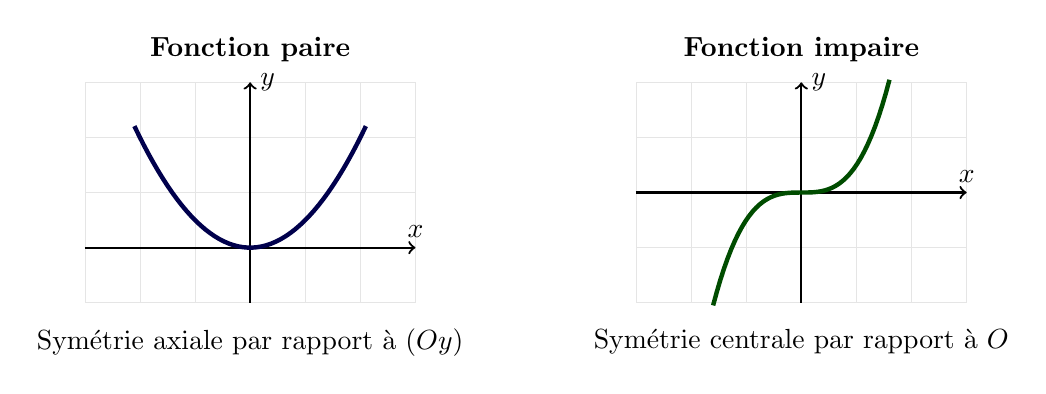
\begin{tikzpicture}[scale=0.7]
		\begin{scope}[xshift=-5cm]
			\draw[very thin, gray!20] (-3,-1) grid (3,3);
			\draw[->, thick] (-3,0) -- (3,0) node[above] {$x$};
			\draw[->, thick] (0,-1) -- (0,3) node[right] {$y$};
			\draw[blue!30!black, ultra thick, domain=-2.1:2.1, samples=50] plot(\x, {0.5*\x*\x});
			\node[above] at (0, 3.2) {\textbf{Fonction paire}};
			\node[below] at (0,-1.3) {Symétrie axiale par rapport à $(Oy)$};
		\end{scope}

		\begin{scope}[xshift=5cm,yshift=1cm]
			\draw[very thin, gray!20] (-3,-2) grid (3,2);
			\draw[->, thick] (-3,0) -- (3,0) node[above] {$x$};
			\draw[->, thick] (0,-2) -- (0,2) node[right] {$y$};
			\draw[green!30!black, ultra thick, domain=-1.6:1.6, samples=50] plot(\x, {0.5*\x*\x*\x});
			\node[above] at (0, 2.2) {\textbf{Fonction impaire}};
			\node[below] at (0,-2.3) {Symétrie centrale par rapport à $O$};
		\end{scope}
	\end{tikzpicture}
\end{center}

\newpage

\begin{methode}[Étudier la parité d'une fonction]
	Étudier la parité des fonctions définies sur $\R$ :
	\begin{multicols}{3}
		\begin{itemize}
			\item $f(x) = x^4 - 3x^2$
			\item $g(x) = \dfrac{2x}{x^2 + 1}$
		\end{itemize}
	\end{multicols}

	\begin{correction}
		\nline
		\begin{itemize}
			\item $\R$ est symétrique par rapport à $0$. Pour tout $x \in \R$ :
			      \[
				      f(-x) = (-x)^4 - 3(-x)^2 = x^4 - 3x^2 = f(x)
			      \]

			      La fonction $f$ est donc \textbf{paire}.
			\item $\R$ est symétrique par rapport à $0$. Pour tout $x \in \R$ :
			      \[
				      g(-x) = \dfrac{2(-x)}{(-x)^2 + 1} = \dfrac{-2x}{x^2 + 1} = -\pa{\dfrac{2x}{x^2 + 1}} = -g(x)
			      \]

			      La fonction $g$ est donc \textbf{impaire}.
		\end{itemize}
	\end{correction}
\end{methode}

\section{Variations et extrema}

\subsection{Sens de variation}

\begin{defin}[Croissance et décroissance]
	Soit $f$ une fonction définie sur un intervalle $I$.
	\begin{itemize}
		\item $f$ est \textbf{strictement croissante} sur $I$ si pour tous réels $a, b \in I$ tels que $a < b$, on a $f(a) < f(b)$.
		\item $f$ est \textbf{strictement décroissante} sur $I$ si pour tous réels $a, b \in I$ tels que $a < b$, on a $f(a) > f(b)$.
	\end{itemize}
\end{defin}

\begin{rem}
	\nline
	\begin{itemize}
		\item Une fonction \textbf{croissante} conserve l'ordre.
		\item Une fonction \textbf{décroissante} inverse l'ordre.
		\item Une fonction est dite \textbf{monotone} sur un intervalle $I$ si elle y est uniquement croissante ou uniquement décroissante.
	\end{itemize}
\end{rem}

\subsection{Extrema : Maximum et Minimum}

\begin{defin}[Maximum et minimum]
	Soit $f$ une fonction définie sur un intervalle $I$ et $x_0 \in I$.
	\begin{itemize}
		\item $f$ admet un \textbf{maximum} en $x_0$ sur $I$ si pour tout $x \in I$, $f(x) \le f(x_0)$. Ce maximum vaut $M = f(x_0)$.
		\item $f$ admet un \textbf{minimum} en $x_0$ sur $I$ si pour tout $x \in I$, $f(x) \ge f(x_0)$. Ce minimum vaut $m = f(x_0)$.
	\end{itemize}
\end{defin}

\subsection{Tableau de variations}

Un \textbf{tableau de variations} résume le sens de variation de la fonction $f$ ainsi que ses extrema locaux et aux bornes.

\begin{methode}[Dresser et exploiter un tableau de variations]
	Soit la fonction $f$ définie sur $[-5\,;\,6]$ dont le tableau de variations est donné ci-dessous.

	\begin{center}
		\begin{tikzpicture}
			\tkzTabInit[lgt=1.5, espcl=1.8, deltacl=0.5]{$x$ /1, $f(x)$ /2}{$-5$, $-1$, $3$, $6$}
			\tkzTabVar{-/ $-4$, +/ $5$, -/ $-2$, +/ $1$}
		\end{tikzpicture}
	\end{center}

	\begin{enumerate}
		\item Donner le sens de variation de $f$.
		\item Déterminer le maximum et le minimum de $f$ sur $\intff{-5}{6}$.
		\item Comparer, si possible, $f(-4)$ et $f(-2)$.
	\end{enumerate}

	\begin{correction}
		\nline
		\begin{enumerate}
			\item $f$ est strictement croissante sur $\intff{-5}{-1}$ et $\intff{3}{6}$, et strictement décroissante sur $\intff{-1}{3}$.
			\item Le maximum absolu de $f$ est $5$, atteint en $x = -1$. Le minimum absolu est $-4$, atteint en $x = -5$.
			\item Sur $\intff{-5}{-1}$, les nombres $-4$ et $-2$ sont rangés dans l'ordre $-5 \le -4 < -2 \le -1$.

			      Comme $f$ est \textbf{strictement croissante} sur cet intervalle, elle conserve l'ordre :
			      \[
				      f(-4) < f(-2)
			      \]
		\end{enumerate}
	\end{correction}
\end{methode}

\section{Résolutions graphiques et positions relatives}

\subsection{Équations et inéquations de la forme $f(x) = k$ et $f(x) \ge k$}

\begin{prop}[Résolution graphique]
	Soit $f$ une fonction définie sur $\mathcal{D}$ de courbe $\Cf$, et $k \in \R$.
	\begin{itemize}
		\item Les solutions de l'équation $f(x) = k$ sont les \textbf{abscisses} des points d'intersection de la courbe $\Cf$ avec la droite horizontale d'équation $y = k$.
		\item Les solutions de l'inéquation $f(x) > k$ (resp. $f(x) < k$) sont les \textbf{abscisses} des points de la courbe $\Cf$ situés \textbf{strictement au-dessus} (resp. au-dessous) de la droite $y = k$.
	\end{itemize}
\end{prop}

\begin{methode}[Résoudre graphiquement $f(x) = k$ et $f(x) \ge k$]
	On considère la fonction $f$ représentée par sa courbe $\Cf$ ci-dessous.

	\begin{center}
		\begin{tikzpicture}[scale=0.75]
			\draw[very thin, gray!40] (-3.5,-2.5) grid (3.5,3.5);
			\draw[-{Stealth}, thick] (-3.5,0) -- (3.5,0) node[above] {$x$};
			\draw[-{Stealth}, thick] (0,-2.5) -- (0,3.5) node[right] {$y$};
			\foreach \x in {-3,-2,-1,1,2,3} \node[below=1pt, font=\small, fill=white] at (\x,0) {\x};
			\foreach \y in {-2,-1,1,2,3} \node[left=1pt, font=\small, fill=white] at (0,\y) {\y};
			\node[below left, font=\small] at (0,0) {0};
			\draw[blue, ultra thick, samples=100, domain=-3.2:3.2] plot(\x, {0.5*\x*\x - 2}) node[above right] {$\Cf$};
			\draw[red, thick] (-3.5,2) -- (3.5,2) node[right] {$y = 2$};
			\filldraw (-2.83,2) circle (2.5pt);
			\filldraw (2.83,2) circle (2.5pt);
			\draw[dashed, thick] (-2.83,0) -- (-2.83,2);
			\draw[dashed, thick] (2.83,0) -- (2.83,2);
		\end{tikzpicture}
	\end{center}

	Résoudre graphiquement sur $\intff{-3}{3}$ :

	\begin{enumerate}
		\item L'équation $f(x) = 2$.
		\item L'inéquation $f(x) \ge 2$.
	\end{enumerate}

	\begin{correction}
		\nline
		\begin{enumerate}
			\item On trace la droite horizontale d'équation $y = 2$.

			      Elle coupe la courbe $\Cf$ en deux points d'abscisses $-2{,}8$ et $2{,}8$.

			      L'ensemble des solutions de l'équation $f(x) = 2$ est :
			      \[
				      S = \{-2{,}8\,;\,2{,}8\}
			      \]

			\item Les solutions de l'inéquation $f(x) \ge 2$ sont les abscisses des points de la courbe $\Cf$ situés \textbf{au-dessus ou sur} la droite d'équation $y = 2$.

			      L'ensemble des solutions est :
			      \[
				      S = \intff{-3}{-2{,}8} \cup \intff{2{,}8}{3}
			      \]
		\end{enumerate}
	\end{correction}
\end{methode}

\subsection{Résolution de $f(x) = g(x)$ et position relative de deux courbes}

\begin{prop}[Comparaison de deux fonctions]
	Soit $f$ et $g$ deux fonctions de courbes représentatives $\Cf$ et $\Cg$.
	\begin{itemize}
		\item Les solutions de $f(x) = g(x)$ sont les \textbf{abscisses} des points d'intersection de $\Cf$ et $\Cg$.
		\item $\Cf$ est \textbf{au-dessus} de $\Cg$ sur un intervalle si et seulement si $f(x) \ge g(x)$, soit $f(x) - g(x) \ge 0$.
		\item $\Cf$ est \textbf{en dessous} de $\Cg$ sur un intervalle si et seulement si $f(x) \le g(x)$, soit $f(x) - g(x) \le 0$.
	\end{itemize}
\end{prop}

\begin{methode}[Résoudre graphiquement une inéquation du type $f(x) < g(x)$]
	\nline
	\begin{wrapstuff}[r]
		\begin{tikzpicture}[scale=0.85]
			\draw[very thin, black!40] (-1.5,-0.5) grid (4.5,6.5);
			\draw[-{Stealth}, black, thick] (-1.5,0) -- (4.5,0) node[right] {$x$};
			\draw[-{Stealth}, black, thick] (0,-0.5) -- (0,6.5) node[above] {$y$};
			\foreach \x in {-1,1,2,3} \node[below=1pt, font=\small, black, fill=white] at (\x,0) {\x};
			\foreach \y in {1,2,3,4,5,6} \node[left=1pt, font=\small, black, fill=white] at (0,\y) {\y};

			\draw[cyan!60!black, ultra thick, samples=100, domain=-1.3:2.2] plot(\x,{\x*\x+2}) node[below right] {$\Cf$};
			\draw[green!60!black, ultra thick, samples=100, domain=-0.7:3.7] plot(\x,{-\x*\x+3*\x+2}) node[right] {$\Cg$};

			\filldraw[red!30!black] (0,2) circle (2.5pt);
			\filldraw[red!30!black] (1.5,4.25) circle (2.5pt);

			\draw[dashed, red!30!black, thick] (0,0) -- (0,2);
			\draw[dashed, red!30!black, thick] (1.5,0) -- (1.5,4.25);
		\end{tikzpicture}
	\end{wrapstuff}

	On a représenté les courbes $\Cf$ et $\Cg$ des fonctions :

	\begin{itemize}
		\item $f(x) = x^2 + 2$
		\item $g(x) = -x^2 + 3x + 2$
	\end{itemize}

	Résoudre graphiquement $f(x) < g(x)$.

	\ms

	\noindent\textit{Correction :}

	L'inéquation $f(x) < g(x)$ correspond aux valeurs de $x$ pour lesquelles $\Cf$ est \textbf{strictement au-dessous} de $\Cg$.

	Les deux courbes se coupent aux points d'abscisses $x = 0$ et $x = 1{,}5$.

	$\Cf$ est située en dessous de $\Cg$ entre ces deux valeurs.

	L'ensemble des solutions est donc :
	\[
		S = \left] 0\,;\,1{,}5 \right[
	\]
\end{methode}

\subsection{Tableau de signes}

Le \textbf{tableau de signes} permet de déterminer sur quels intervalles une fonction est positive ($f(x) \ge 0$), négative ($f(x) \le 0$) ou s'annule ($f(x) = 0$).

\begin{methode}[Dresser un tableau de signes graphiquement]
	Dresser le tableau de signes de la fonction $h$ représentée ci-contre sur $\intff{-3{,}5}{2{,}2}$.
	\begin{center}
		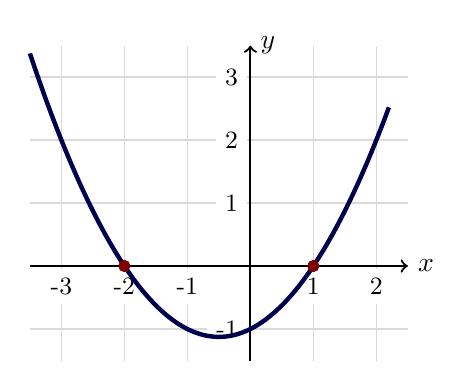
\begin{tikzpicture}[scale=0.80]
			\draw[thin, gray!30] (-3.5,-1.5) grid (2.5,3.5);
			\draw[->, thick] (-3.5,0) -- (2.5,0) node[right] {$x$};
			\draw[->, thick] (0,-1.5) -- (0,3.5) node[right] {$y$};
			\foreach \x in {-3,-2,-1,1,2} \node[below=1pt, font=\small, fill=white] at (\x,0) {\x};
			\foreach \y in {-1,1,2,3} \node[left=1pt, font=\small, fill=white] at (0,\y) {\y};
			\draw[blue!30!black, ultra thick, samples=100, domain=-3.5:2.2] plot (\x, {0.5*(\x+2)*(\x-1)});
			\filldraw[red!50!black] (-2,0) circle (2.5pt);
			\filldraw[red!50!black] (1,0) circle (2.5pt);
		\end{tikzpicture}
	\end{center}

	\begin{correction}
		$\mathcal{C}_h$ coupe l'axe des abscisses en $x = -2{,}7$ et $x = 0{,}7$.

		La courbe est au-dessus de l'axe sur $\intff{-3{,}5}{-2}$ et $\intff{1}{2{,}2}$, et au-dessous sur $\intff{-2}{1}$.
		\begin{center}
			\begin{tikzpicture}
				\tkzTabInit[lgt=1.5, espcl=1.8]{$x$ /1, $h(x)$ /1}{$-3{,}5$, $-2$, $1$, $2{,}2$}
				\tkzTabLine{, +, z, -, z, +, }
			\end{tikzpicture}
		\end{center}
	\end{correction}
\end{methode}
